\documentclass[9pt,onecolumn,twoside]{pnas-new}
% Use the lineno option to display guide line numbers if required.
% Note that the use of elements such as single-column equations
% may affect the guide line number alignment. 

\usepackage{mathtools}
\usepackage{subcaption}
\captionsetup[subfigure]{justification=justified,singlelinecheck=false}

\setboolean{displaywatermark}{false}

\templatetype{pnasresearcharticle} % Choose template 
% {pnasresearcharticle} = Template for a two-column research article
% {pnasmathematics} = Template for a one-column mathematics article
% {pnasinvited} = Template for a PNAS invited submission

\title{Topological Fractal Dimension of Protein-Protein Interaction Networks}
% Use letters for affiliations, numbers to show equal authorship (if applicable) and to indicate the corresponding author
\author[]{Mahan Ghafari}
\author[]{Rocco Meli}
\author[]{Florian Störtz}

\affil[]{Interdisciplinary Bioscience DTP, Rex Richards Building, University of Oxford, Oxford OX1 3RQ}

% Please give the surname of the lead author for the running footer
\leadauthor{Ghafari} 

% Please add here a significance statement to explain the relevance of your work
% \significancestatement{} (not needed for BioDTP)

% Please include corresponding author, author contribution and author declaration information
%\authorcontributions{Please provide details of author contributions here.}
%\authordeclaration{Please declare any conflict of interest here.}
%\equalauthors{\textsuperscript{1}A.O.(Author One) and A.T. (Author Two) contributed equally to this work (remove if not applicable).}
%\correspondingauthor{\textsuperscript{2}To whom correspondence should be addressed. E-mail: author.two\@email.com}

% Keywords are not mandatory, but authors are strongly encouraged to provide them. If provided, please include two to five keywords, separated by the pipe symbol, e.g:
\keywords{Topological Fractal Dimension $|$ Protein-Protein Interaction Networks} 

\begin{abstract}
Protein-protein interaction networks are attracting increasingly more attention in recent years thanks to the rapid development of new methods to study protein structures, functions, and interactions. These networks provide a level of abstraction that enables us to understand some of the global features of protein interactions in cells. A large number of them exhibit scale-free and scale-invariant behavior. Here, we measure the fractal dimension of some real cellular networks using three different box counting methods. We also put forward a new method for measuring fractal dimension based on the box burning method. We find that a power-law relation between the number of
boxes needed to cover the networks and the size of the boxes does indeed exist, and subsequently compare the performance and limitations of each method.
\end{abstract}

\dates{\today}

\begin{document}

% Optional adjustment to line up main text (after abstract) of first page with line numbers, when using both lineno and twocolumn options.
% You should only change this length when you've finalised the article contents.
\verticaladjustment{-2pt}

\maketitle
\thispagestyle{firststyle}
\ifthenelse{\boolean{shortarticle}}{\ifthenelse{\boolean{singlecolumn}}{\abscontentformatted}{\abscontent}}{}

% If your first paragraph (i.e. with the \dropcap) contains a list environment (quote, quotation, theorem, definition, enumerate, itemize...), the line after the list may have some extra indentation. If this is the case, add \parshape=0 to the end of the list environment.
\dropcap{P}rotein-protein interactions (PPIs) are the basis of many important cellular processes such as signal transduction, molecular transport and various metabolism pathways. 
Aberrant PPIs are responsible for many aggregation-related diseases, such as Alzheimer's disease \cite{kramer2012}, and may also lead to cancer \cite{liu2011}. Understanding PPIs is also essential in drug development, since drugs can affect them by manipulating active sites of proteins. 
Therefore, they have been studied extensively in the area of bioscience and medical research \cite{oti2006, ivanov2013, laraia2015}. 
Proteins interact with each other on a physical level due to the combined effects of hydrophobic bonding, salt bridges and van der Waals forces at specific binding domains. Their interaction has several biochemical effects \cite{phiz1995,srinivasa2014}, which can be used for detection: they can alter the kinetic properties of enzymes affecting their binding to substrates, create new binding sites, inactivate a protein or result in a new function that neither interaction partner had before.
Early methods like yeast two-hybrid screening \cite{fields1989} relied on the latter effect, i.e.\ the altering of gene expression in a reporter gene mediated by the interaction of two specific proteins \emph{in vivo}. The method had first been established for \emph{Saccharomyces cerevisiae}, which therefore offers the most extensive data set to date \cite{biogrid2017}.
The development of large-scale PPI screening techniques, especially high-throughput affinity purification combined with mass spectrometry \cite{yates2009}, 
has caused an explosion in the amount of PPI data and the construction of ever more complex and complete interactomes, i.e.\ the totality of PPIs that happen in cells and organisms. This method involves the selective purification of a tagged protein and its interaction partners, and subsequent analysis via mass spectrometry.
Our current knowledge of interactomes is both incomplete and noisy, as all the current PPI detection methods have their limitations as to how many truly physiological interactions they can detect. Experimental results have since been catalogued and curated for several online databases \cite{pedamallu2014, biogrid2017} in the form of single undirected interaction data points.

Protein-protein interaction networks (PPINs) are mathematical representations of the physical contacts between proteins in the cell. 
These contacts are specific binding regions in the protein that serve a specific function. 
Knowledge of PPIs enables us to assign putative roles to uncharacterized proteins, add fine-grained detail about the steps within a signalling pathway, and characterize the relationships between proteins that form multi-molecular complexes such as the proteasome \cite{embl_networkanalysis}.
Understanding the structure of these interaction networks only provides one dimension of the biochemical machinery controlling cell behavior. Apart from cellular networks, one might also study metabolic networks \cite{zhu2005structural}, gene expression networks \cite{bergmann2003similarities}, and domain interaction networks \cite{wuchty2006stable}.

Due to the great level of connectivity between proteins, PPINs demonstrate small-world effects.
This means that, no matter how big the PPIN is, the maximum number of steps separating any two protein interactions (i.e.\ nodes in the network) is small.
Several studies have shown that real complex networks, ranging from the world wide web to protein-protein interaction networks, 
have self-repeating patterns over a wide range of length scales \cite{song2004, concas2006, song2007}.

In this work, we first import protein interactions from the BioGRID online database (\url{https://www.thebiogrid.org/}, build 3.5.165 of 23rd Sep 2018) \cite{biogrid2017}, into the Python network manipulation package \texttt{networkx}. To unfold the self-similar properties of PPINs, we then calculate their topological fractal dimension using several possible box covering algorithms \cite{song2004,concas2006,song2007,zhang2014}. 
We also put forward a new method for calculating the topological fractal dimension using the `burning method'. 
We then compare these methods against some generic network structures as well as cellular networks of \emph{Escherichia coli} and \emph{Arabidopsis thaliana}. 
Finally, we discuss the results and compare the limitations and efficiency of each method.

\section*{Data Import and Analysis}
\begin{table}
\centering
\caption{\textmd{Definitions}} \label{tab:symbols} 
\begin{tabular}{l p{.4\textwidth}}
\hline
Term              & Definition \\
\hline
Node (or vertex)    & A protein in a network \\
Edge (or link)    & Functional (or physical) interaction between proteins \\
Degree    & The number of incoming/outgoing edges \\
Hub  & A node with a high degree\\
Shortest path length  & Smallest number of steps (edges) to connect a pair of nodes\\
Diameter & Maximum shortest path length in the network\\
Local diameter nodes & All nodes separated from a local starting node by equal length  \\
\hline
\end{tabular}
\end{table}

The Python library \texttt{pandas} was used to import BioGRID files into a \texttt{networkx} graph. The latter automatically cleaned the data. An execution time analysis of this process is depicted in Figure~\ref{fig:runtime_buildgraph}, showing a power law dependence of the execution time on the number of edges $M$ across several orders of magnitude.

\begin{figure}
    \centering
    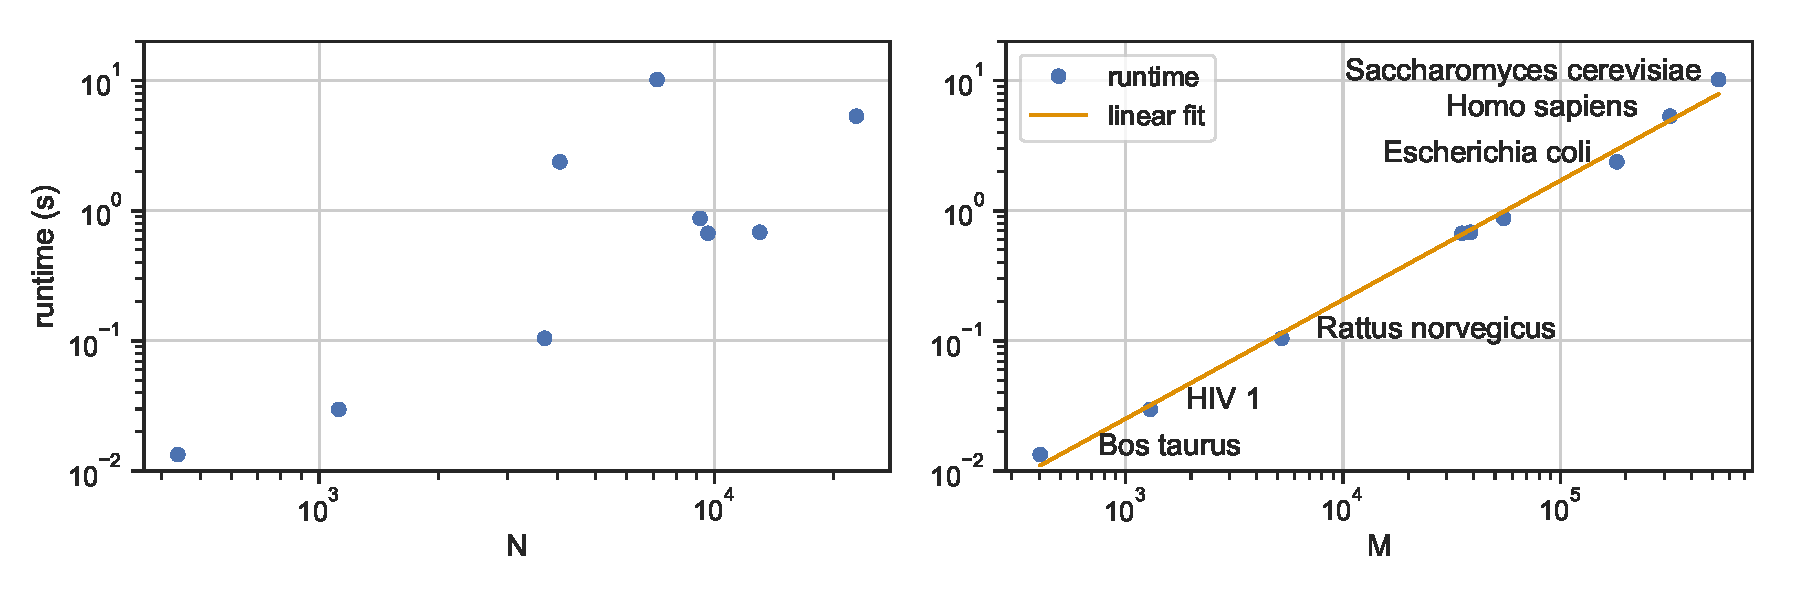
\includegraphics[width=0.9\columnwidth]{images/runtimes_loadgraph_annotated.pdf}
    \caption{Runtime analysis of building the graphs from the BioGRID files for several organisms using the Python library \texttt{networkx}. This involves deletion of selfloops and duplicates in the graph. We observe a power law dependence of the runtime on the number of edges $M$, whereas the dependence on the number of nodes $N$ is not as uniform.}
    \label{fig:runtime_buildgraph}
\end{figure}

%Betweenness centrality quantifies the number of times a node acts as a bridge along the shortest path between two other nodes
%\textcolor{red}{Plot network graph, compute centrality measures. Describe betweenness, eigenvector and pagerank}
In order to quantify the importance of a node, we calculated three centrality measures for each node (see Figures~\ref{fig:rat_centrality} and \ref{fig:homosapiens_centrality}). Betweenness quantifies how often a node is part of the shortest path between two other nodes, eigenvector centrality is the sum over the eigenvector centrality of neighboring nodes, and the PageRank value, which in an undirected graph as ours is proportional to the degree of a node \cite{grolmusz2015}. 

\begin{figure}
\centering
\begin{subfigure}{.42\textwidth}
    \centering
    \vspace{2.2em}
    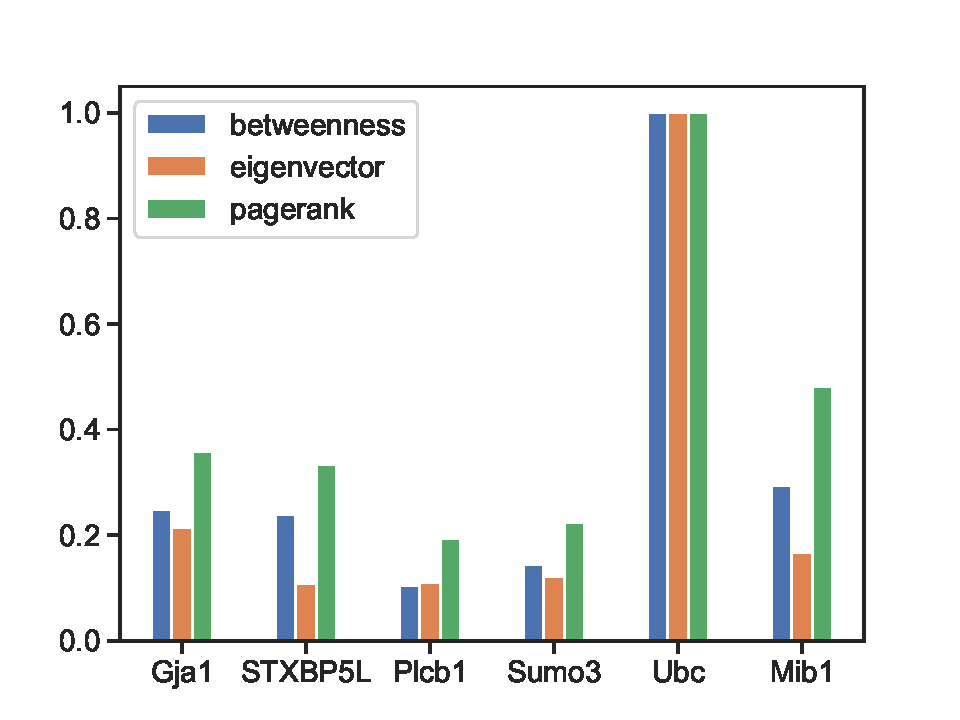
\includegraphics[width=\columnwidth]{images/rat_centrality.pdf}
    \vspace{1.1em}
    \caption{}
    \label{fig:rat_centrality}
\end{subfigure}%
\begin{subfigure}{.58\textwidth}
    \centering
    \vspace{-1em}
    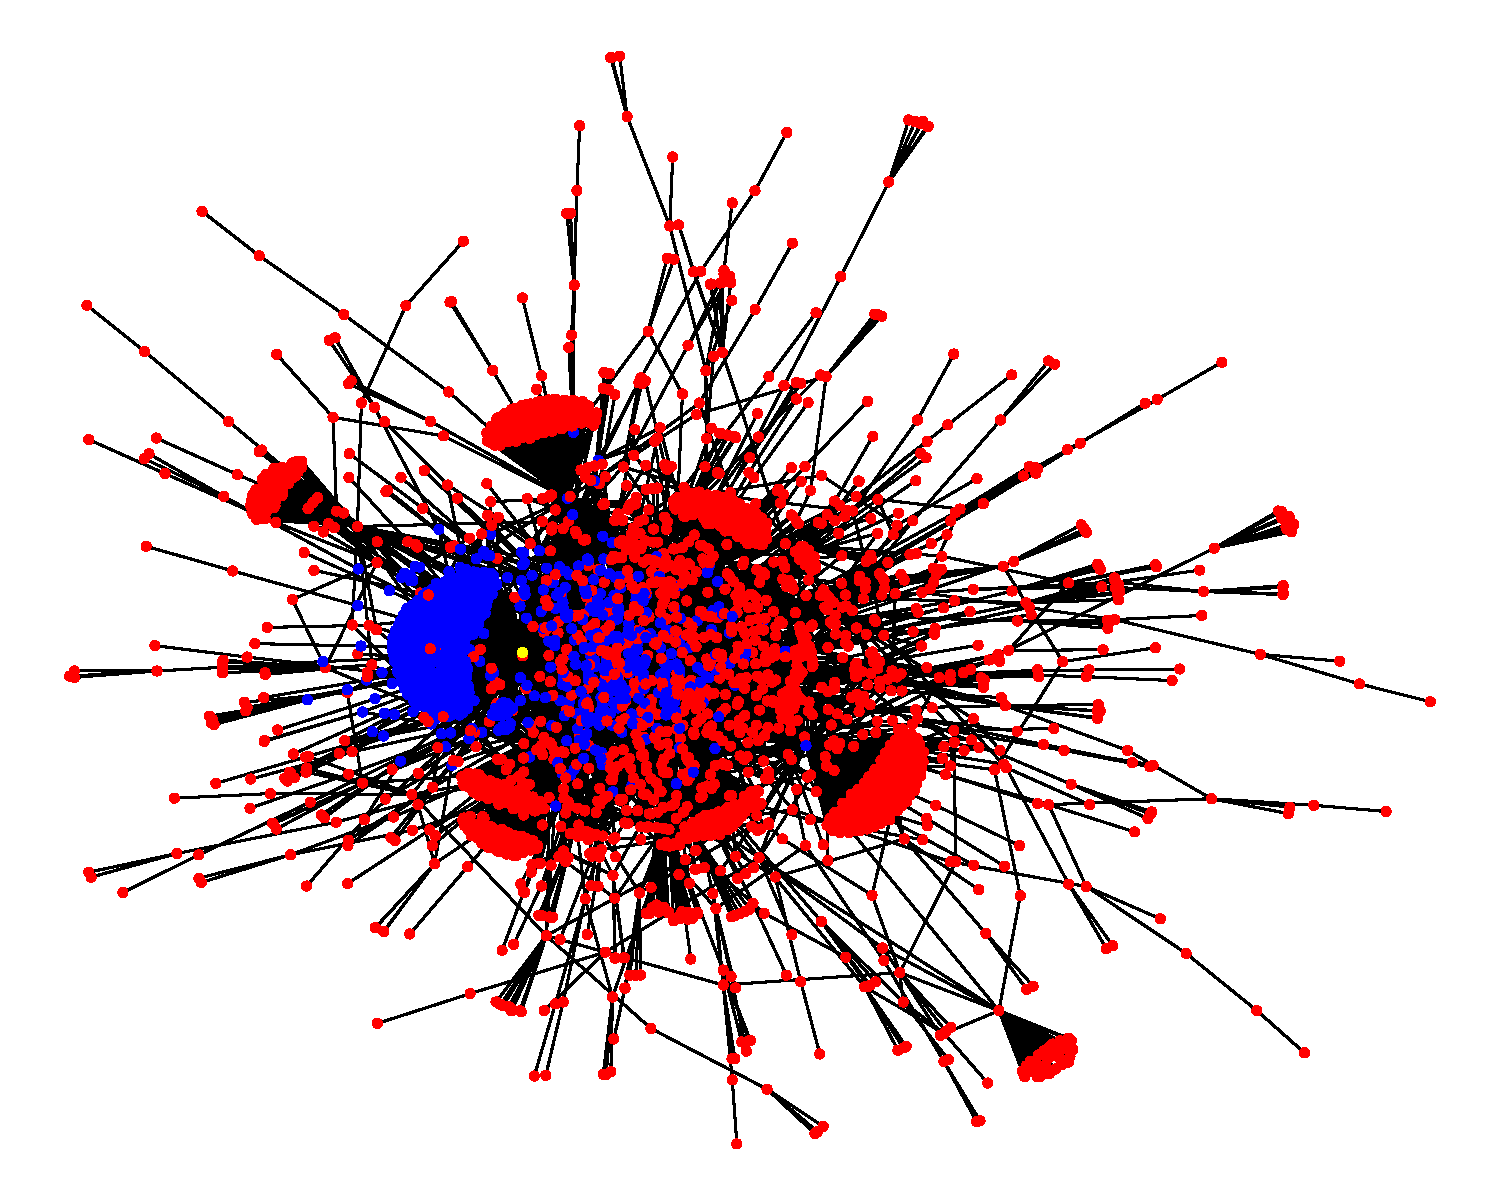
\includegraphics[width=\columnwidth]{images/rat_network.pdf}
    \vspace{-2.7em} 
    \caption{}
    \label{fig:rat_network}
\end{subfigure}
\caption{Network analysis of the protein interactions in \emph{Rattus norvegicus}, the biggest part of which were obtained experimentally in Reference \cite{na2013}. \textbf{a)} Centrality measures for the highest-scoring proteins, where the values have been normalized such that the maximum score for each measure equals unity. For the PageRank centrality, we chose a damping factor of $\alpha = 0.85$. The Ubiquitin-C (Ubc) protein is the most central for all three measures. \textbf{b)} Visualization of the largest connected component (3254 proteins with 5013 interactions). The central part is densely interconnected, with several distinct bunching points, and shows outgoing interaction chains. The yellow dot in the center-left region represents the Ubc protein which is the most central in the network; blue dots represent proteins which immediately interact with Ubc.}
\label{fig:test}
\end{figure}

Figure \ref{fig:rat_centrality} shows the Ubiquitin-C (Ubc) protein to be the one with the highest centrality in \emph{Rattus norvegicus} by our chosen measures. The reason for this is that it is frequently found in covalent bonds with other proteins or even itself (polyubiquitin chains) and, depending on its binding partner, can assist in DNA repair, cell-cycle regulation, endocytosis and catabolic processes in muscle cells \cite{price2002}.

\begin{figure}
    \centering
    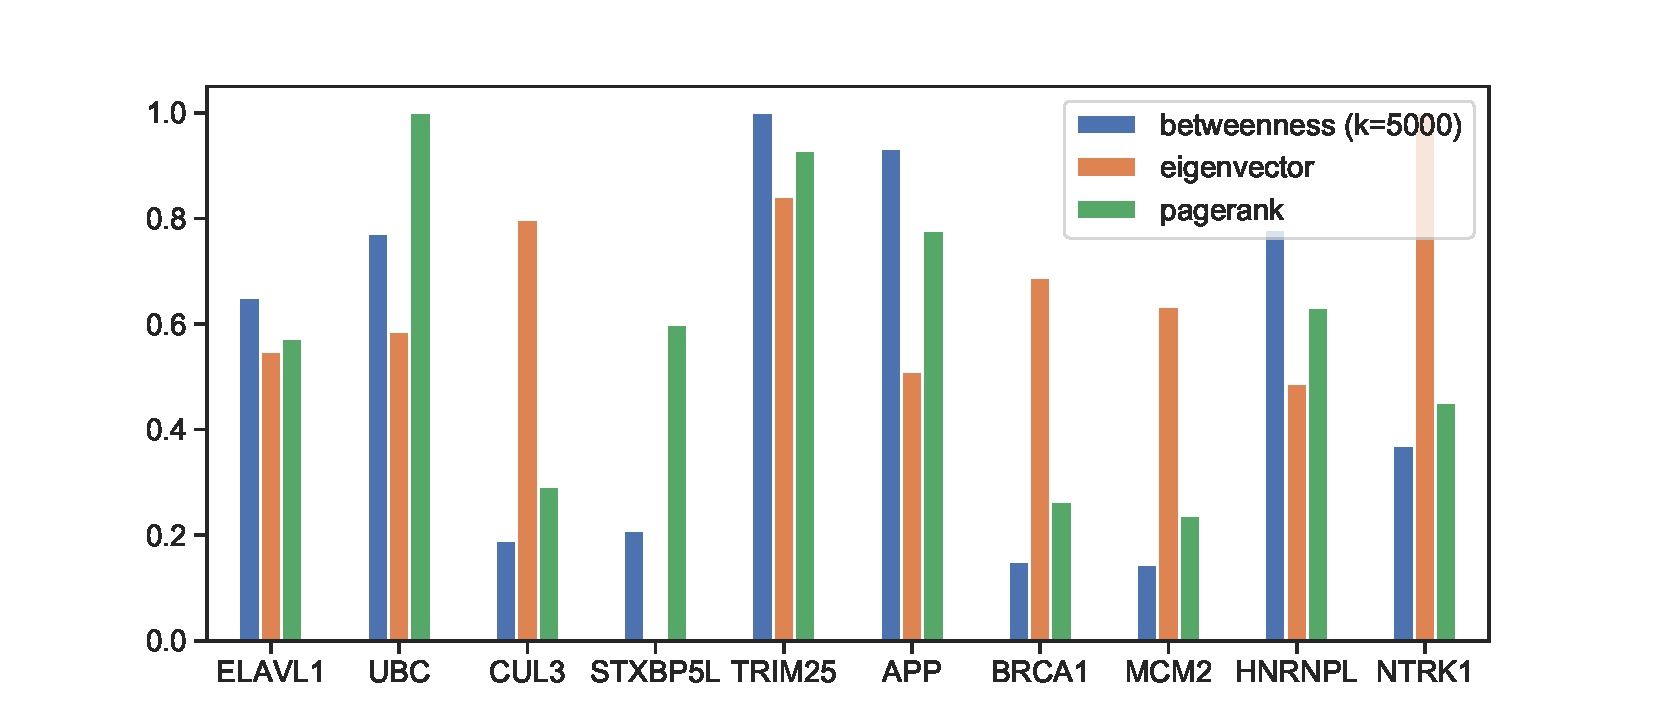
\includegraphics[width=0.8\columnwidth]{images/homosapiens_centrality.pdf}
    \caption{Centrality measures for \emph{H. sapiens}. As it is computationally costly, we only used $k=5000$ randomly sampled nodes when evaluating the betweenness of each node.}
    \label{fig:homosapiens_centrality}
\end{figure}

Figure \ref{fig:homosapiens_centrality} shows the same centrality measures for the highest scoring human proteins. We observe that the TRIM25 protein, whose RING-type region is involved in viral immune defense \cite{jung2007}, has the highest overall centrality. NTRK1, which is a nerve growth factor receptor, has the highest eigenvector centrality and has a pro-survival signalling effect in neurons \cite{ginty2011}. Together with CUL3, it has been shown to act as a hub protein \cite{shafiee2018}.

\section*{Box-covering Algorithm}
In order to compute the fractal dimension $d$ of a network, we use a box-covering algorithm. The idea behind a  box-covering algorithm is to find the minimum number of boxes of a given size needed to cover all the nodes of the complex network. 
The fractal dimension of a complex networks relates the minimum number of boxes $N_B$ and the size of the box $l_B$ as
\begin{equation}
    N_B\sim l_B^{-d}.
    \label{eq:fractal}
\end{equation}
Therefore, in order to compute the fractal dimension of a network we have to compute $N_B$  for different values of $l_B$ and perform a power-law fit in order to obtain $d$.  

In this work, we implemented three different methods to compute the fractal dimension of a network: the burning algorithm, the greedy coloring algorithm and the fuzzy algorithm. 

\begin{figure}
    \centering
    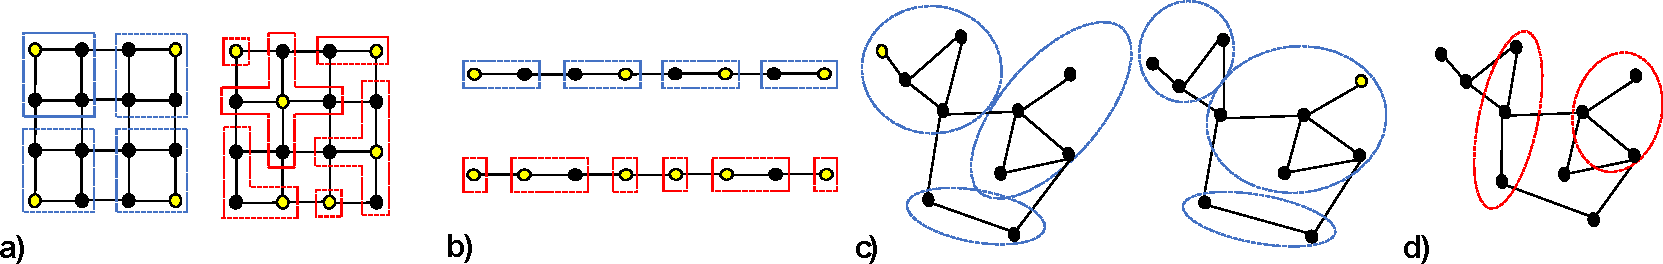
\includegraphics[width=1.\columnwidth]{images/starting_node.pdf}
    \caption{Counting the number of boxes in \textbf{a)} a lattice and \textbf{b)} a path network. Yellow points show the starting nodes of a compact box (dashed lines). If the starting point is from nodes with the least number of neighbors, the total number of compact boxes (blue lines) is minimum. On the other hand, if the starting nodes are selected randomly, the total number of boxes (red lines) could be higher. Panel \textbf{c)} shows that the total number of boxes tends to stay the same (minimum) as we randomly select different starting points with the least number of neighbors. Panel \textbf{d)} shows an example of making non-compact boxes (red lines).}
    \label{fig:starting_node}
\end{figure}

\section*{Effect of Selecting a Starting Node on the Total Number of Boxes}
To obtain an estimate for the fractal dimension, we have to ensure that the total number of boxes (or colors) is minimal. One way to test this is to see how $N_B$ changes with the starting node of a compact box of length $l_B$. Figure \ref{fig:starting_node} shows why picking a node with the least number of neighbors can provide a smaller number of boxes than randomly selecting nodes to form compact boxes. We put this into test by comparing the two strategies in estimating the fractal dimension of a lattice (see Figure~\ref{fig:comparing_startingNodes}). We find that the fractal dimension of a random model $d \approx 1.60$ is less accurate than selecting nodes with minimum adjacent neighbors, for which we obtain $d \approx 1.75$. Additionally, the distribution of box counts tends to be much more spread around the mean for the former method.

\begin{figure}
    \centering
    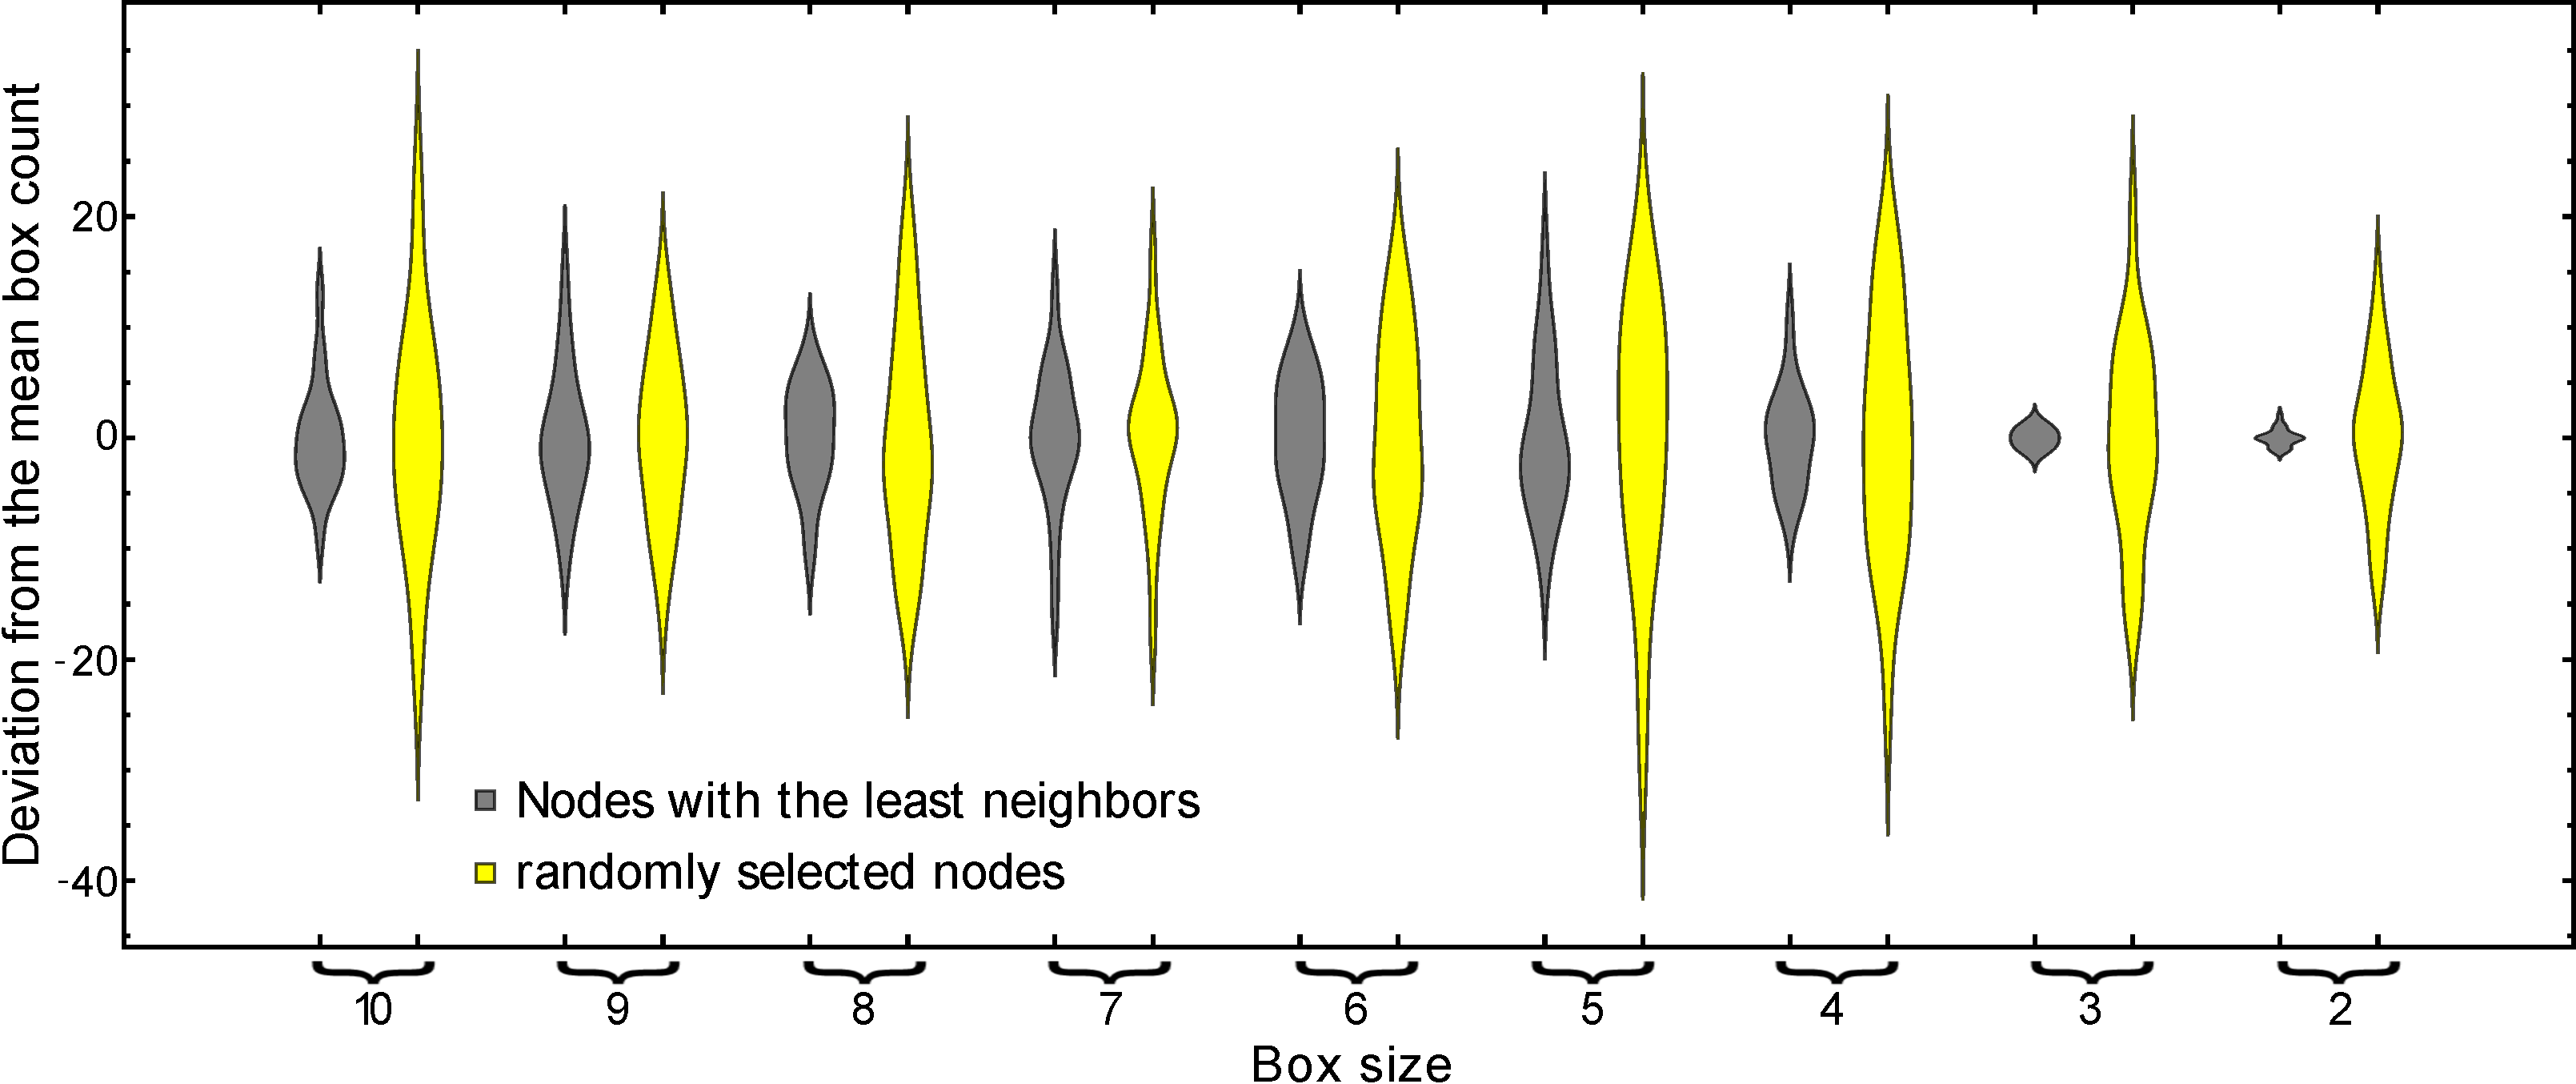
\includegraphics[width=0.75\columnwidth]{images/decent_comparison.pdf}
    \caption{The effect of choosing the initial node of a compact box on the total box count. For a $50 \times 50$ lattice, we count the minimum number of boxes by randomly selecting nodes in the lattice (gray) and randomly selecting nodes with the least number of neighbors (yellow) to form the minimum set of compact boxes. We run 20 independent simulations and vary the box size from 10 to 2 to get a distribution over the total number of boxes using each approach (for a box size of length 1, the total box count will be equal to the total number of nodes in the lattice, i.e. 2500). We find that the variation in the total number of boxes is much higher for randomly selected nodes.}
    \label{fig:comparing_startingNodes}
\end{figure}


\section*{Finite-Size Effects}
In order to test our algorithms, we apply them to two simple networks: a linear and a lattice network (see Figure~\ref{fig:lattice_and_path}). For the linear network we expect an integer dimension $d_\text{expected}=1$ while for the lattice network we expect an integer dimension $d_\text{expected}=2$. When we apply the algorithms to these networks, we found that the fractal dimensions are smaller than the expected dimensions.

To investigate this behaviour we applied the fuzzy algorithm to networks with an increasing number of nodes, the results of which are reported in Figure~\ref{fig:fse}. We see that when increasing the linear number of nodes (the number of nodes for the linear network and the square root of the number of nodes for the lattice network), the normalized fractal dimension $d/d_\text{expected}$ approaches the correct limit. However the convergence rate decreases, as can be inferred from Figure~\ref{fig:fse}.

Finally, to better understand this phenomenon and see whether it is related to the finite size of the networks, we applied periodic boundary conditions (PBCs). These are commonly employed to simulate infinite systems \cite{kittel2004} and therefore we expect such boundary conditions to lower the extent of finite-size effects. As we can see from Figure~\ref{fig:fse} this is indeed the case: the use of periodic boundary conditions shifts the fractal dimension towards the expected limit. Surprisingly, the use of periodic boundary conditions does not seem to increase the convergence rate with respect to the linear number of nodes.

\begin{figure}[h]
    \centering
    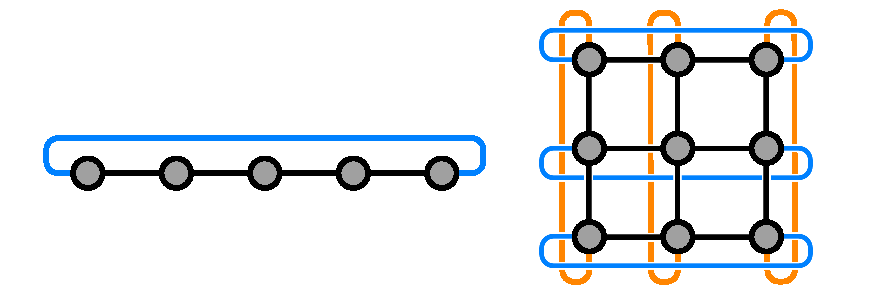
\includegraphics[width=0.5\columnwidth]{images/path_lattice.pdf}
    \caption{\textbf{(Left)} Linear (or path) network with $N = 5$ nodes and \textbf{(right)} Lattice network with $N=9$ nodes. Black lines represent the edges without periodic boundary conditions, i.e. the path network is just a 1D line and the lattice network is a 2D grid. Colored lines represent the edges added to obtain periodic boundary conditions: topologically, the path network becomes a ring while the lattice network becomes a torus.}
    \label{fig:lattice_and_path}
\end{figure}

\begin{figure}
    \centering
\begin{subfigure}{.5\textwidth}
    \centering
    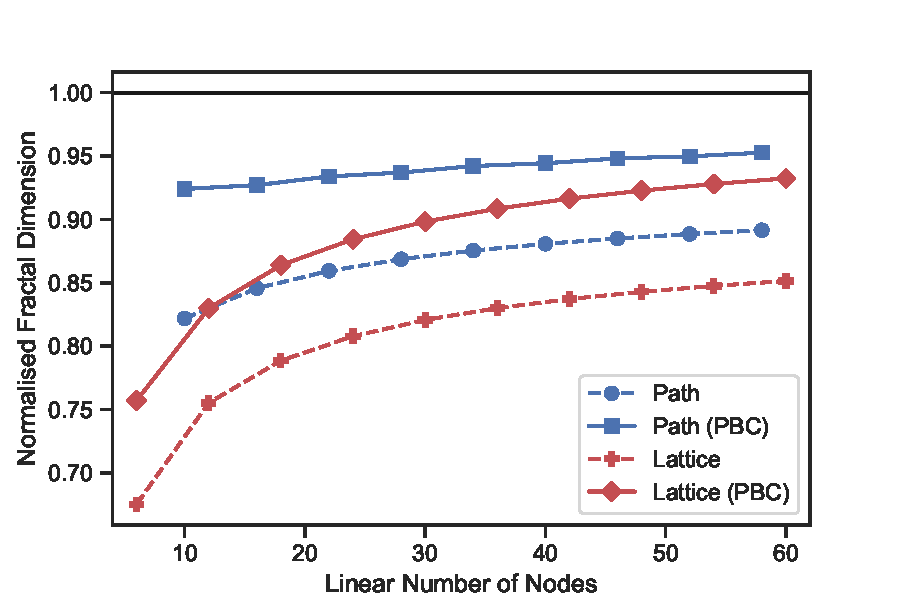
\includegraphics[width=\columnwidth]{images/fse.pdf}
    \caption{}
    \label{fig:fse}
\end{subfigure}%
\begin{subfigure}{.5\textwidth}
    \centering
    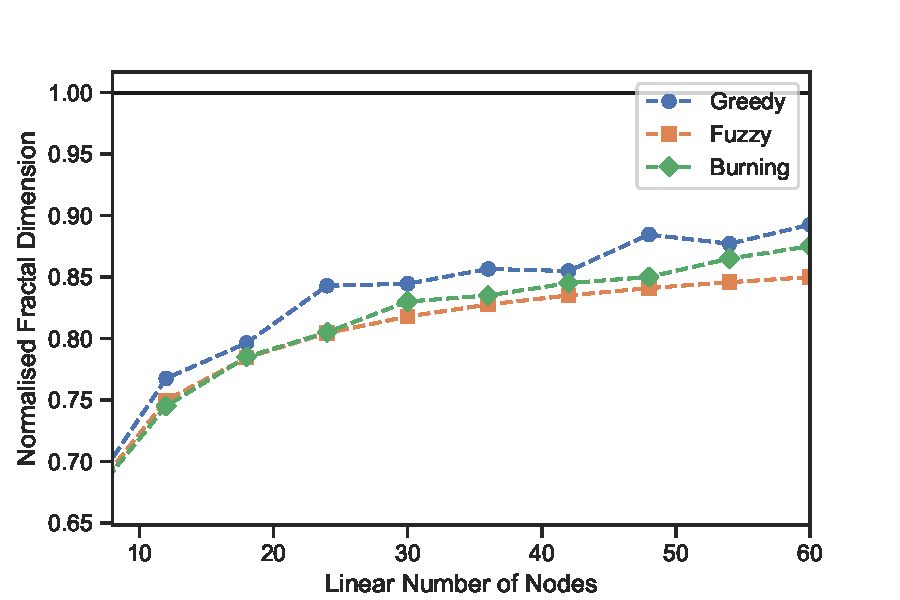
\includegraphics[width=\columnwidth]{images/fse_comparison.pdf}
    \caption{}
    \label{fig:algos}
\end{subfigure}
    \caption{\textbf{(a)} Finite-size effects for path and lattice graphs. The fractal dimension of both graphs slowly converges to the exact limit $d/d_\text{expected} = 1$ with an increasing number of nodes. The use of periodic boundary conditions improves the fractal dimension, providing a vertical shift towards the exact limit, but does not appear to improve the convergence rate. \textbf{(b)} Normalized fractal dimension $d/2$ for a lattice network (without periodic boundary conditions) as a function of the linear number of nodes in the lattice for the three different algorithms (burning, fuzzy and greedy).}
    \label{fig:fseALL}
\end{figure}

\section*{Comparison of Different Methods to Compute the Fractal Dimension of a Network}
We implemented three different algorithms:  the burning method \cite{song2004,concas2006,song2007}, the greedy coloring algorithm \cite{song2007} and the fuzzy algorithm \cite{zhang2014}, comparing their relative performance.

Figure~\ref{fig:algos} shows the normalized fractal dimension $d/2$ for a lattice graph (without periodic boundary conditions) as a function of the linear number of nodes in the lattice for the three different algorithms. We see that for the lattice graph, they give a comparable fractal dimension and have a similar trend. This result shows that for networks with a simple structure the three algorithms produce identical results.

The greedy algorithm was run only once and therefore we could not perform averaging. This accounts for the fluctuations observed for the greedy algorithm in Figure~\ref{fig:algos}, since the algorithm is not deterministic \cite{song2007} and an average over a large number of runs is expected to yield more accurate results.

\section*{Fractal Dimension $d$ of Real Protein-Protein Interaction Networks}
After testing our algorithms and their properties, we applied them to real protein-protein interaction data obtained from the BioGRID database. Table~\ref{tab:results} reports the fractal dimensions we obtained using three different algorithms: a novel box burning (based on Refs.~\cite{song2004,concas2006,song2007}), a greedy coloring \cite{song2007} and the fuzzy method \cite{zhang2014}.

From Table~\ref{tab:results}, we see that the fractal dimensions obtained with the three different algorithms do not always match as expected. Despite the three algorithms giving very similar results for the path and lattice networks, when applied to real networks the results are not as close. This suggests that path and lattice graphs may be `too simple' to yield differences between the three algorithms. The other major issue is that we need a larger sampling pool to report the mean fractal dimension and standard deviations reliably. Also, for the power law behavior to emerge (see Equation \ref{eq:fractal}), we need at least an order of magnitude change in the range of box size. This was impossible to obtain for some networks, like \textit{E.\ coli}, or computationally costly for some algorithms, like the Box Burning method. The Burning method also demands relatively high RAM usage (approx.\ 20 GB for \emph{E.\ coli}) which necessitated the use of a High Performance Computing cluster to generate some of the results on cellular networks.

The fuzzy method uses a completely different approach to the computation of networks' fractal dimension from the other two methods and therefore we can expect some deviations depending on the particular structure of the network. However, we expect the greedy algorithm and the burning algorithm to give similar results. Apart from \emph{Human herpesvirus 8} this is not quite the case. This can be explained by the fact that the greedy algorithm uses a larger range of box lengths $l_B$ (from 1 to the diameter of the network) while the burning method only uses boxes up to roughly half of the diameter. We expect that including a larger range of box lengths would improve the results from burning method, but this was not possible due to the computational complexity of the algorithm.

Table~\ref{tab:results} also compares our results to other works in the literature. Given the high and increasing number of databases for biological networks, people tend to use different databases and different versions for PPINs. Only two of the results obtained by Wang \emph{et al.}\ uses the same BioGRID database. The original paper by Song \emph{et al.}\ \cite{song2007} studies a metabolic network in \emph{E.\ coli} (instead of a PPIN). This, combined with the use of different algorithms, makes the comparison with the literature quite challenging. 
%However the range of fractal dimension for PPIN (that usually have small-world and scale-free feature) is comparable.

\begin{table}
\centering
\caption{\textmd{Fractal Dimension $d$ for different PPINs with comparison values. Only the values marked with $\star$ are known to stem from BioGRID data.}} \label{tab:results} 
\begin{tabular}{l | c c | c c c | c c c c}
\hline
Organism & $N$ & $M$ & Fuzzy & Burning & Greedy & Song \emph{et al.}\ \cite{song2004} & Wang \emph{et al.}\ \cite{anh2011} & Wei \emph{et al.}\ \cite{wei2013} & Jin \emph{et al.}\ \cite{jin2013}\\
\hline
\emph{Human herpesvirus 8}      & 714   & 687       & 2.30 & 2.20 & 2.32 &  &  &  &\\
\emph{Caenorhabditis elegans}   & 3,953  & 7,885      & 3.86 & 1.39 & 2.31 & & 3.48 $\pm$ 0.24 $\star$  &  1.704 & 1.6$\pm$0.1\\
\emph{Arabidopsis thaliana}     & 9,626  & 35,242    & 4.16 & 1.83 & 2.61 & & 2.26 $\pm$ 0.06 $\star$  &  &1.5$\pm$0.1\\
\emph{Escherichia coli K-12}    & 4,063  & 181,620   & 5.10 & 3.44 & 4.51 & 2.3 & 2.37 $\pm$ 0.11 \,\,\,  &  3.351 & 3.6$\pm$0.3\\
%\emph{Homo sapiens}             & 22,840& 318,912   & &  & & 2.3 & 2.20 $\pm$ 0.09 \,\,\, &  &2.9$\pm$ 0.2\\
\hline
\end{tabular}
\end{table}

 
\matmethods{
\label{sec:fundamentals}
For a network $\mathcal{G}$ and box size $l_B$ a compact box is defined as the set of nodes where all the distances $l_{ij}$ between nodes $i$ and $j$ are smaller than $l_B$ and $N_B$ is the minimum number of boxes needed to cover the entire network $\mathcal{G}$ \cite{Feder1988}. As can be seen from Equation \ref{eq:fractal}, the fractal dimension $d$ of the network $\mathcal{G}$  is obtained by a linear fit of $log(N_B)$ versus $\log(l_B)$.

\noindent In this section we will briefly review and describe the different methods we used to compute the minimum number of boxes $N_B$ of size $l_B$ needed to cover a given network  $\mathcal{G}$.

\subsection*{Greedy Coloring Fractal Dimension}
Song \emph{et al.}\ showed that the problem of finding the minimum number of boxes $N_B$ for a given box size $l_B$ can be mapped to a coloring problem \cite{song2007}, a well known NP-hard problem in graph theory \cite{garey1979}. 

In order to compute $N_B(l_B)$ for a given network $\mathcal{G}$ using Song's greedy coloring algorithm, one has to compute the dual network $\mathcal{G}'$, defined as the network where the nodes of the original network $\mathcal{G}$ are connected if their distance in $\mathcal{G}$ is greater than or equal to $l_B$. Once the network $\mathcal{G}'$ is computed a vertex coloring algorithm gives the natural number of boxes as the number of colors \cite{song2007}. This is because vertex with the same colors in $\mathcal{G}'$ are at a distances smaller than or equal to $l_B$ in the original network $\mathcal{G}$ and therefore are within the same box. This concept is illustrated in Figure~\ref{fig:gc_algo} for a simple case ($N=6$ nodes, $M=6$ edges and $l_B = 3$).

\begin{figure}
    \centering
    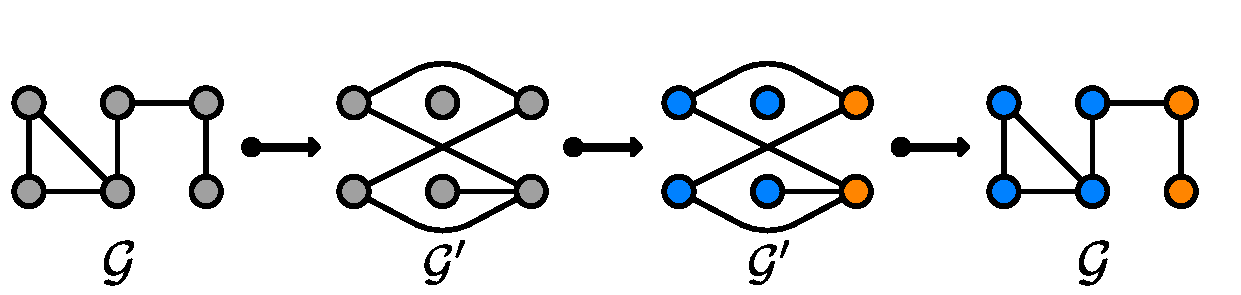
\includegraphics[width=0.65\columnwidth]{images/gc_algo.pdf}
    \caption{Greedy coloring algorithm for box counting of Song \emph{et al.}\ applied to a simple network for $l_B = 3$ \cite{song2007}. The algorithm starts with a network $\mathcal{G}$ and builds the dual network $\mathcal{G}'$ for a given box size $l_B$. A vertex coloring algorithm is applied to the dual network $\mathcal{G}'$ so that no connected vertices have the same color. The color scheme transferred to the original network gives its box covering. Figure adapted from Ref.~\cite{song2007}.}
    \label{fig:gc_algo}
\end{figure}

The vertex coloring problem is an NP-hard problem and therefore a brute-force solution is computationally very expensive \cite{christofides1971}. However, a greedy coloring algorithm can give a good approximation of this problem in reasonable time \cite{song2007}. The drawbacks of this approach is that the results are dependent on the choice of the starting node, therefore some statistics has to be performed.

The naive implementation of Song's algorithm (calculation of all shortest paths, explicit construction of the dual network, greedy coloring) requires the construction of the dual network for every box length $l_B$, which is an $\mathcal{O}(N^2)$ operation. However, Song \emph{et al.}\ suggest a very efficient implementation that only needs a single network pass \cite{song2007}.

\subsection*{Fuzzy Fractal Dimension}
In order to overcome the limitations of the greedy coloring algorithm, Zhang \emph{et al.}\ proposed a fuzzy method to calculate the inverse of the minimum number of boxes of a given size in order to cover a graph $\mathcal{G}$ \cite{zhang2014}. The idea behind this algorithm is to use spherical boxes that can actually overlap, in order to find the covering ability, i.e.\ the inverse of the minimum number of boxes, for a given box size $l_B$.

In the fuzzy fractal dimension method, balls of radius $l_B$ are constructed around each node of the given network $\mathcal{G}$, and the inverse of the minimum number of boxes (the covering ability) needed to cover the graph for a given size is given by
\[
    N^{-1}(l_B) = \frac{1}{N(N-1)} \sum_{i}^N \sum_{j\neq i}^N \Omega_{ij}(l_B)A_{ij}(l_B)
\]
where
\[
    \Omega_{ij}(l_B) = \begin{cases} 1,& \quad d_{ij} \le l_B \\ 0,& \quad \text{otherwise} \end{cases} \qquad \mathrm{and} \qquad A_{ij} = \exp\left( -\frac{d_{ij}^2}{l_B^2} \right).
\]
As usual, $d_{ij}$ is the shortest path between nodes $i$ and $j$. $\Omega_{ij}$ is a connectivity factor describing whether the ball centered at node $i$ can cover node $j$, and $A_{ij}$ is a measure of how well the ball centered at node $i$ can cover node $j$.

The algorithm suggested by Zhang \emph{et al.}\ computes the coverage ability $N_i^{-1}(l_B) = \sum_{j\neq i} \Omega_{ij}(l_B)A_{ij}$ for every node $i$ in the network $\mathcal{G}$ for a given $l_B$. The overall coverage ability is simply the average of such values \cite{zhang2014}. For the network of Figure~\ref{fig:gc_algo} with $l_B=3$, we have \cite{zhang2014}
\[
    N_1^{-1}(3) = 0.594, \quad N_2^{-1}(3) = 0.594, \quad N_3^{-1}(3) = 0.739, \quad  N_4^{-1}(3) = 0.743, \quad  N_5^{-1}(3) = 0.633, \quad N_6^{-1}(3) = 0.448,
\]
so that the final coverage ability for $l_B = 3$ is the average $N^{-1}(3) = 0.625$. This means that the number of boxes with size $l=3$ needed to cover the network is $N(3)=1.6$. This result is similar to the one obtained with the algorithm of Song \emph{et al.}\ but the method is much easier to implement and is fully deterministic so that no averaging over multiple runs is needed.

\subsection*{Burning Algorithm}

This method, first proposed in Reference~\cite{song2004}, tiles the network with boxes of size $l_B$. All the nodes within a box should be `reachable' by a distance smaller than the given $l_B$ (i.e. the box should be compact). Once the compact box is formed, all the nodes inside are burned and the total number of boxes increase by 1. The same protocol continues until all the nodes in the network are removed.

\subsubsection*{(i) Traditional Compact-Box-Burning (CBB) algorithm}

This method was first introduced by Song \emph{et al.}\ \cite{song2007} and can be summarized as follows:
(1) Construct a set $S$ of all yet uncovered nodes. 
(2) Choose a random node in $S$ and remove it from the set. 
(3) Take all nodes whose distance from the initial node is less than the box size $l_B$ and remove them from $S$ (compactness of the box). 
(4) Repeat steps (2) and (3) until the set $S$ is empty. 

One of the drawbacks of this method is that to form each compact box, it has to go through all the nodes in the network and test whether they belong to the same box. This makes the code substantially slow. Furthermore, it starts by picking a random node in the network. As we discussed in the results section, this introduces random fluctuations in fractal dimension estimates which have to be averaged out by running the code several times to obtain a reliable result. For these two reasons, we propose a new method that addresses these issues. 

\subsubsection*{(ii) A Novel Box Burning Algorithm}

This new approach that we developed aims at resolving the issues raised by the traditional CBB algorithm. We apply the following steps in computing the minimum number of boxes (see Figure \ref{fig:box-burning}):
(1) Randomly select a node $p$ out of all the ones that have the lowest number of immediate neighbors. 
(2) Find all the Local Diameter nodes (see Table~\ref{tab:symbols}) that are at distance $l_B-1$ away from $p$. Find all the nodes that are in the shortest path from $p$ to the Local Diameter nodes and store them in a set $S$. 
(3) For each node $i$ in $S$, find all the neighboring nodes $s'_i$ that are at distance $l_i \leq l_B-1$ away from $i$ and store them in a set $s'_i \in S'$. 
(4) Find a set $s^* \in S'$ with the least number of nodes and define it to be the `Minimum Box'. 
(5) Find the intersection over all elements $s'_i$ in $S'$. If that has more nodes than the Minimum Box, remove all of them from the network and go back to step (1). 
If the intersection has fewer nodes than the Minimum Box, remove one node from the Local Diameter of node $p$ and go back to step (2). Continue until all the nodes are removed.

\begin{figure}
    \centering
    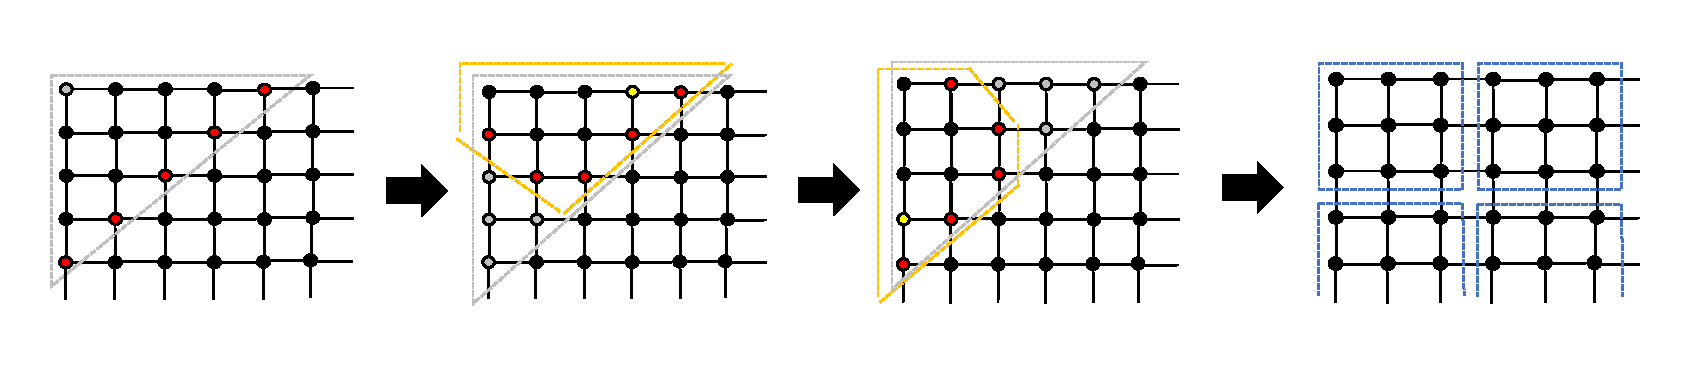
\includegraphics[width=1.03\columnwidth]{images/new_burning.pdf}
    %\vspace{-3.5em}
    \vspace{-2.5em}
    \caption{A novel box-burning method. First, we randomly select a node with the least number of neighbors (yellow node). Then, find the local diameter nodes (red nodes) and form a box around all the nodes inside the local diameter (gray dashed line). Then, we go through each node inside the gray box and find all the nodes within the local diameter nodes (yellow dashed lines) and store the list. Finally, we take the intersection of all the yellow boxes and if it is bigger than the size of the minimum box, then we form the box and burn the nodes inside.}
    \label{fig:box-burning}
\end{figure}

} % matmethods

\showmatmethods % Display the Materials and Methods section

\acknow{The authors thank Dr.\ Florian Klimm for fruitful discussions about the project.}

\showacknow % Display the acknowledgments section
%\subsection*{Author Affiliations}

\section*{Feedback}
Working on this project we learned about PPINs and how graph theory can be applied to such networks in order to better understand their properties. This is an intriguing field and the project was entertaining while being challenging. However, we found that the literature is somewhat confusing, with different authors using different methods and datasets so that a comparison within the field is not always trivial.

During this project we spent some time learning new concepts in programming and software engineering. We realized how version control helps collaborating on a code base on GitHub (\url{github.com}) and tried to apply some software engineering practices. In particular, we used the Python test framework \texttt{pytest} and we set up continuous integration using Travis-CI (\url{travis-ci.org}) so that the test suite is run for every commit. We also set up code coverage on CodeCov (\url{codecov.io}), which helped to spot missing tests and dummy code.


%Include department, institution, and complete address, with the ZIP/postal code, for each author. Use lower case letters to match authors with institutions, as shown in the example. Authors with an ORCID ID may supply this information at submission.
% \pnasbreak splits and balances the columns before the references.
% If you see unexpected formatting errors, try commenting out this line
% as it can run into problems with floats and footnotes on the final page.
\pnasbreak

% Bibliography
\bibliography{references}

\end{document}